%%%%%%%%%%%%%%%%%%%%%%%%%%%%%%%%%%%%%%%%%%%%%%%%%%%%%%%%%%%%%%%%%%%%%%%%%%%%%%%%
%nscience.tex: Chapter on theory:
%%%%%%%%%%%%%%%%%%%%%%%%%%%%%%%%%%%%%%%%%%%%%%%%%%%%%%%%%%%%%%%%%%%%%%%%%%%%%%%%
\chapter{Physics of the Standard Model and Left-Right Symmetric Extensions}
\label{ch:theory}

\section{Development of the Standard Model}

The standard model of particle physics, or simply the standard model, encapsulates discoveries in physics stretching well over a century and was chiefly formulated by Weinberg, Glashow, and Salam \cite{PhysRevLett.19.1264}\cite{nla.cat-vn956113}.  The standard model combines electromagnetism, the nuclear weak force, and the nuclear strong force to describe the properties and interactions of all matter, excluding gravity.

At the beginning of the 20th century, Einstein and Lorentz developed special relativity. Maxwell's early work developing the four equations of electricity and magnetism was shown to be fundamentally Lorentz invariant, valid in all reference frames \cite{1898KNAB1427L}\cite{doi:10.1002/andp.19053221004}.  In the 1920s Dirac created the first quantum field-theory, recreating Maxwell's equations for relativistic and quantum cases \cite{doi:10.1098/rspa.1928.0023}.  With this reformulation, the first new particles, anti-particles, were predicted and the fundamental spin of particles was explained.  Dirac's predictions were confirmed by Anderson in 1932 when cosmic-rays were observed decaying to oppositely charged electrons (anti-electrons, or positrons) \cite{PhysRev.43.491}.  Then in the 1940s Feynman developed Quantum Electrodynamics (QED) and with the work of others created a completely-consistent theory of all electromagnetic interactions \cite{PhysRev.76.769}.

The weak nuclear force was first motivated by beta decay.  Pauli noticed a lack of conservation of momentum in the decay, necessitating an extremely light and unseen particle, which was called ``little neutral one'', or neutrino.  This allowed for momentum conservation and Fermi proposed a contact interaction between a proton, electron, and the neutrino.  This interaction between four-fermions successfully predicted the spectrum of beta decay \cite{Fermi1934}, though it has since been updated to include the weak boson, only directly observable at much higher energies than nuclear decays.

Into the 1950s further study of the weak force lead to a puzzle regarding the conservation of parity.  Two particles were discovered, \ensuremath{\tau} and \ensuremath{\theta}, which were identical except for their parity \cite{osti_4356004}.  Lee and Yang proposed that these were the same particles, which instead violated parity symmetry in its decay \cite{PhysRev.104.254}.  The measurement of the beta decay of polarized \cobaltsixty by Wu confirmed the parity-violating nature of the weak force \cite{articlePARITYTEST}.  Meson decays in a storage ring were also studied, revealing more evidence for parity violation \cite{articlePARITYFAIL}.  Sudarshan, Marshak, Feynman, and Gell-Mann all worked to develop a new model for the weak force which would include parity-violation.  This was the \vminusa  model, vector minus axial vector. Axial vectors do not transform the same under parity as regular vectors \cite{1898KNAB1427L}\cite{PhysRev.109.193}.

Parallel to the work developing the \vminusa formulation, Yang and Mills created a non-Abelian gauge theory describing the weak force in 1954.  This replaced the contact interaction, first theorized by Fermi, with a charge 1, spin 1 particle as an intermediary \cite{PhysRev.96.191}.  This theory was physically impossible for the weak force, as the weak boson proposed was massless, requiring the weak force to be of infinite range, like electromagnetism.  Glashow modified the proposed theory in 1960.  He added the \vminusa model of Sudarshan and Marshak and combined Feynman's QED, describing it all in a single theory with the gauge group \SUtwoUone \cite{GLASHOW1961579} and predicting an additional heavy boson mixing with the photon.  The weak \SUtwoL group only couples to left-handed chiral states.  The last piece of the puzzle was completed by Weinberg and Salam \cite{PhysRevLett.19.1264}\cite{nla.cat-vn956113}.  They added the Brout, Englert, and Higgs mechanism \cite{PhysRevLett.13.321}\cite{PhysRevLett.13.508} ---which gives mass to vector bosons in the Yang-Mills theory---and predicted an additional boson, the Higgs, not to be discovered until 2012 \cite{higgs2012ATLAS}\cite{higgs2012CMS}.

At the same time as the development of the so called ``electroweak sector'' of the standard model, cosmic rays and nuclear interactions were providing evidence for another fundamental force of a different sort, the strong nuclear force.  Starting in 1947, cosmic ray events studied in cloud chambers led to the discovery of particles such as kaons \cite{1947Natur.160..855R}.  These particles were strange, as they seemed to have an additional quantum number no other particles did.  Gell-Mann and Zweig proposed a symmetry group \SUthree to explain this \cite{osti_4082875} \cite{Zweig:352337}.  This quark model theorized that all strongly interacting particles were composed of fundamental quarks, three observed and one theorized.  The extra property of kaons and other similar mesons, was that they were made partly of ``strange quarks''.  More typical mesons, as well as protons and neutrons, were made of ``up'' and ``down'' quarks.  The theory predicted one more quark, which was discovered and named ``charm''. The theory was later extended to include two more, the ``bottom'' and ``top'' quarks.  The interactions in the quark model are based on color charge and only color neutral particles can be freely propagating.  Adding the \SUthree group to the electroweak sector gives the complete standard model picture, a \SUthreeSUtwoUone symmetry group.

Every particle predicted in the standard model has now been observed.  The first indirect observation of the \Z was in 1973 at CERN \cite{HASERT1973121}.  The charm quark, confirming quark theory, was discovered at BNL and SLAC and then the bottom quark was soon discovered by the E288 experiment \cite{Aubert:1974js}\cite{Augustin:1974xw}\cite{Herb:1977ek}.  In 1983 the weak bosons were directly discovered by the UA1 and UA2 experiments at CERN \cite{Arnison:1983mk}\cite{Bagnaia:1983zx}\cite{Arnison:1983rp}\cite{Banner:1983jy}.  The top quark, the heaviest particle in the standard model, was discovered in 1995 at FNAL by the D0 and CDF groups using the Tevatron \cite{d4eca9bf1d5f49f3a4adc794f80c0a00}\cite{Abachi:1994td}.  Finally, the Higgs boson was first discovered by \CMS and ATLAS at CERN in 2012 with the \LHC.  In addition to the successful discovery of all the particles in the standard model, extremely precise verification of its physical constants have been done.  As an example, the gyromagnetic ratio of the muon has been calculated to within one part in ten billion, and agrees with measurements to better than one part in one billion \cite{PhysRevD.98.030001}.

\section{Components of the Standard Model}
Having followed the historical development of the standard model, let us now take a systematic view of its parts.
The standard model of particle physics combines three of the four discovered fundamental forces in the universe: the electromagnetic force, the weak force, and the strong force.  There has yet to be a successful quantum field theoretic description of gravity, so it is not included.

The standard model describes the fundamental particles and forces in nature with each fundamental force corresponding to a preservation of certain quanta. Each fundamental force is associated with particles which carry the force in exchange between interacting matter, which are charged under the force in question. These interactions in the standard model can be described using Lie algebra, allowing the model to be described as combinations of groups.

\begin{figure}[!btp]
    \centering
    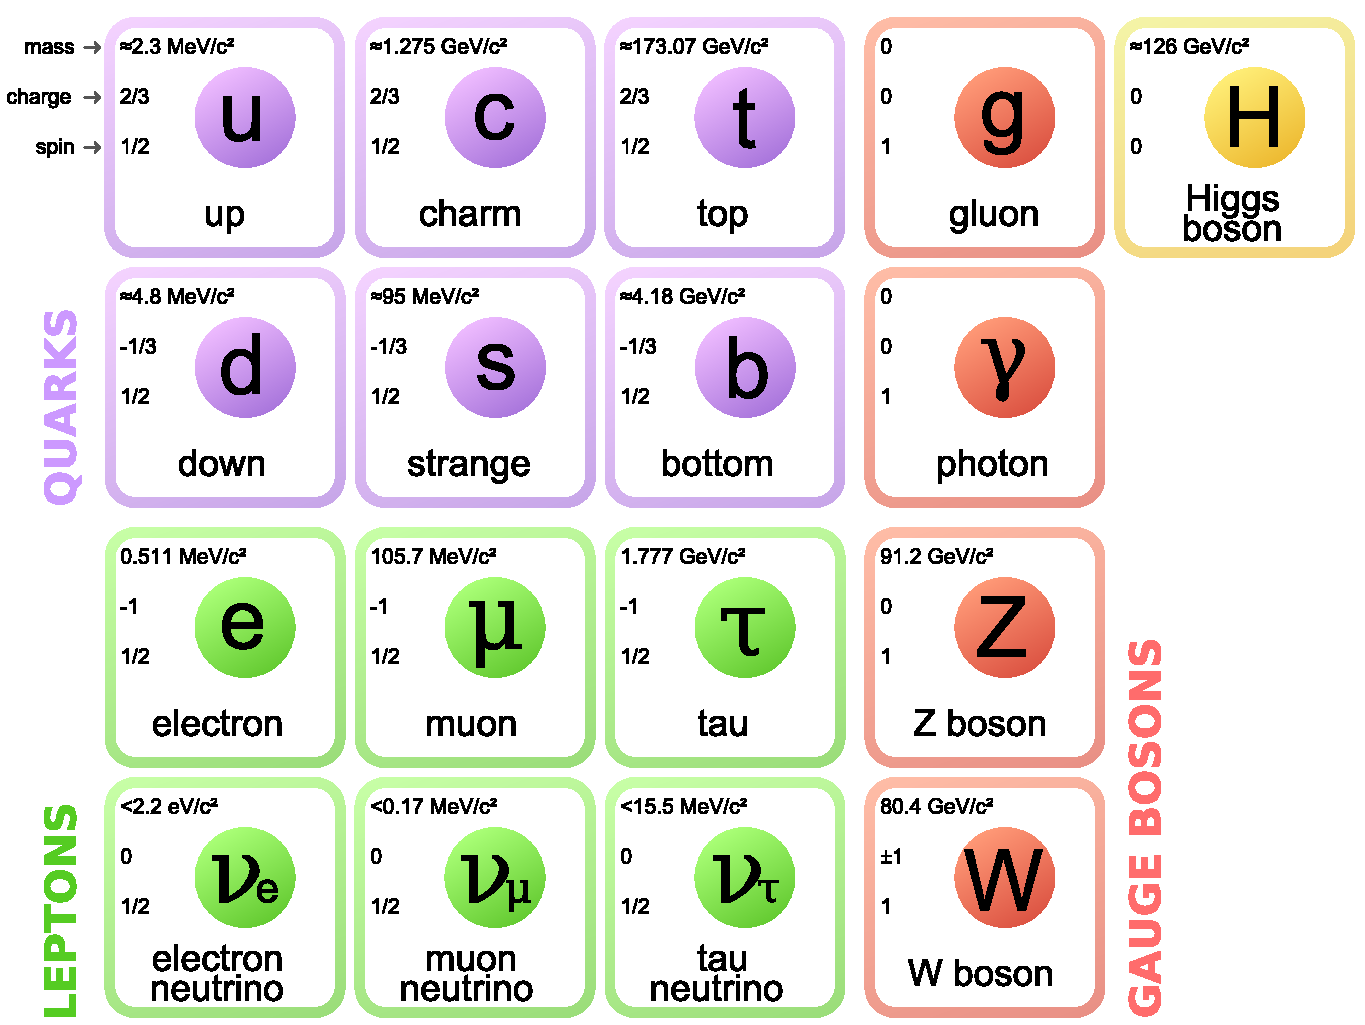
\includegraphics[width=\textwidth]{figures/standard_model.pdf}
    \caption[Diagram of the particles in the standard model.]
       {The particles of the Standard Model.  The quarks are shown in purple, the leptons in green, the exchange particles in red, and the Higgs is shown in yellow.  Each particle's name, mass, charge, and spin is also shown.}
    \label{fig:ParticleTable}
\end{figure}

A diagram of the standard model and each particle's properties is shown in \ref{fig:ParticleTable}.  There are three kinds of particles in the standard model: quarks, leptons, and gauge bosons.  Quarks and leptons make up all of matter and are fermions, while the gauge bosons define the fundamental force interactions and are bosons. There are three generations of quarks and leptons, each heavier than the last.  The lightest generation is the up and down quarks and the electron (and electron neutrino). These particles make up all stable matter in the universe.  Heavier generations have the same charges as these, though they all can decay via the weak force into lighter generations. 

The quarks interact with all of the forces described in the standard model.  They have \ensuremath{\mp\frac{1}{3}} or \ensuremath{\pm\frac{2}{3}} electric charge and a spin of \ensuremath{\frac{1}{2}}. The leptons are the electron, muon, and tau, each with a corresponding neutrino.  Each lepton has a charge of \ensuremath{-1} and a spin of \ensuremath{\frac{1}{2}}.  The neutrinos are not charged however.

At this point it is important to note the unexpected mass distribution in the standard model, which can be read from Fig.~\ref{fig:ParticleTable}. In the first generation of fermions, the up quark and down quark have very similar mass.  From there, the electron has roughly one-quarter of the mass of the down quark. The last particle in the first generation, the electron neutrino, however, has at most one-one-hundred-thousandth of the mass of the others. This significantly smaller mass is difficult to explain naturally and potential sources of the neutrino mass are explained further in section \ref{sec:seesaw}.  

The five bosons of the standard model emerge from the quantum field theories that define it.  The gluon solely interacts with quarks and gluons and is part of the \SUthree group.  The photon (massless) and Z boson (massive) are part of a superposition of weak-flavor neutral fermion-antifermion interactions in the electroweak sector, and the W boson comes from the axial vector, symmetry-breaking part of the electroweak sector.  Its interactions with matter involve weak-flavor transitions, most commonly seen on earth as \ensuremath{\beta}-decay. The Higgs boson, from the Higgs field, gives the weak bosons, W and Z mass, and additionally provides a mechanism for fermion mass.  These interactions will be discussed further in the following subsections.

\subsection{The Strong Force}
\label{sec:QCD}
The strong nuclear force contained in the standard model describes a complicated three flavor interaction \SUthree, described by Quantum Chromodynamics (QCD). Each flavor is described as a ``color'' or ``color charge'': red, green, and blue. Each quark may have one of these colors; anti-quarks have anti-colors. The intermediating particle, the gluon, carries mixtures of color/anti-color. QCD requires the conservation of this color in all interactions. In addition to the conservation of color, free particles must be color neutral (white or black). This feature, called confinement, arises from the fact that as quarks are separated from each other, additional quarks can form from the potential energy in the strong field. This prevents any bare quarks or gluons being visible. Any quark or gluon with sufficient energy to travel away from an interaction will form more colored particles in between it and its past partner. This spray of hadrons is called a ``jet''. Color neutral quark combinations are generally mesons, which are color, anti-color quark pairs, or baryons which are three quark, red-green-blue combinations, all are called hadrons.
\begin{figure}[!btp]
    \centering
    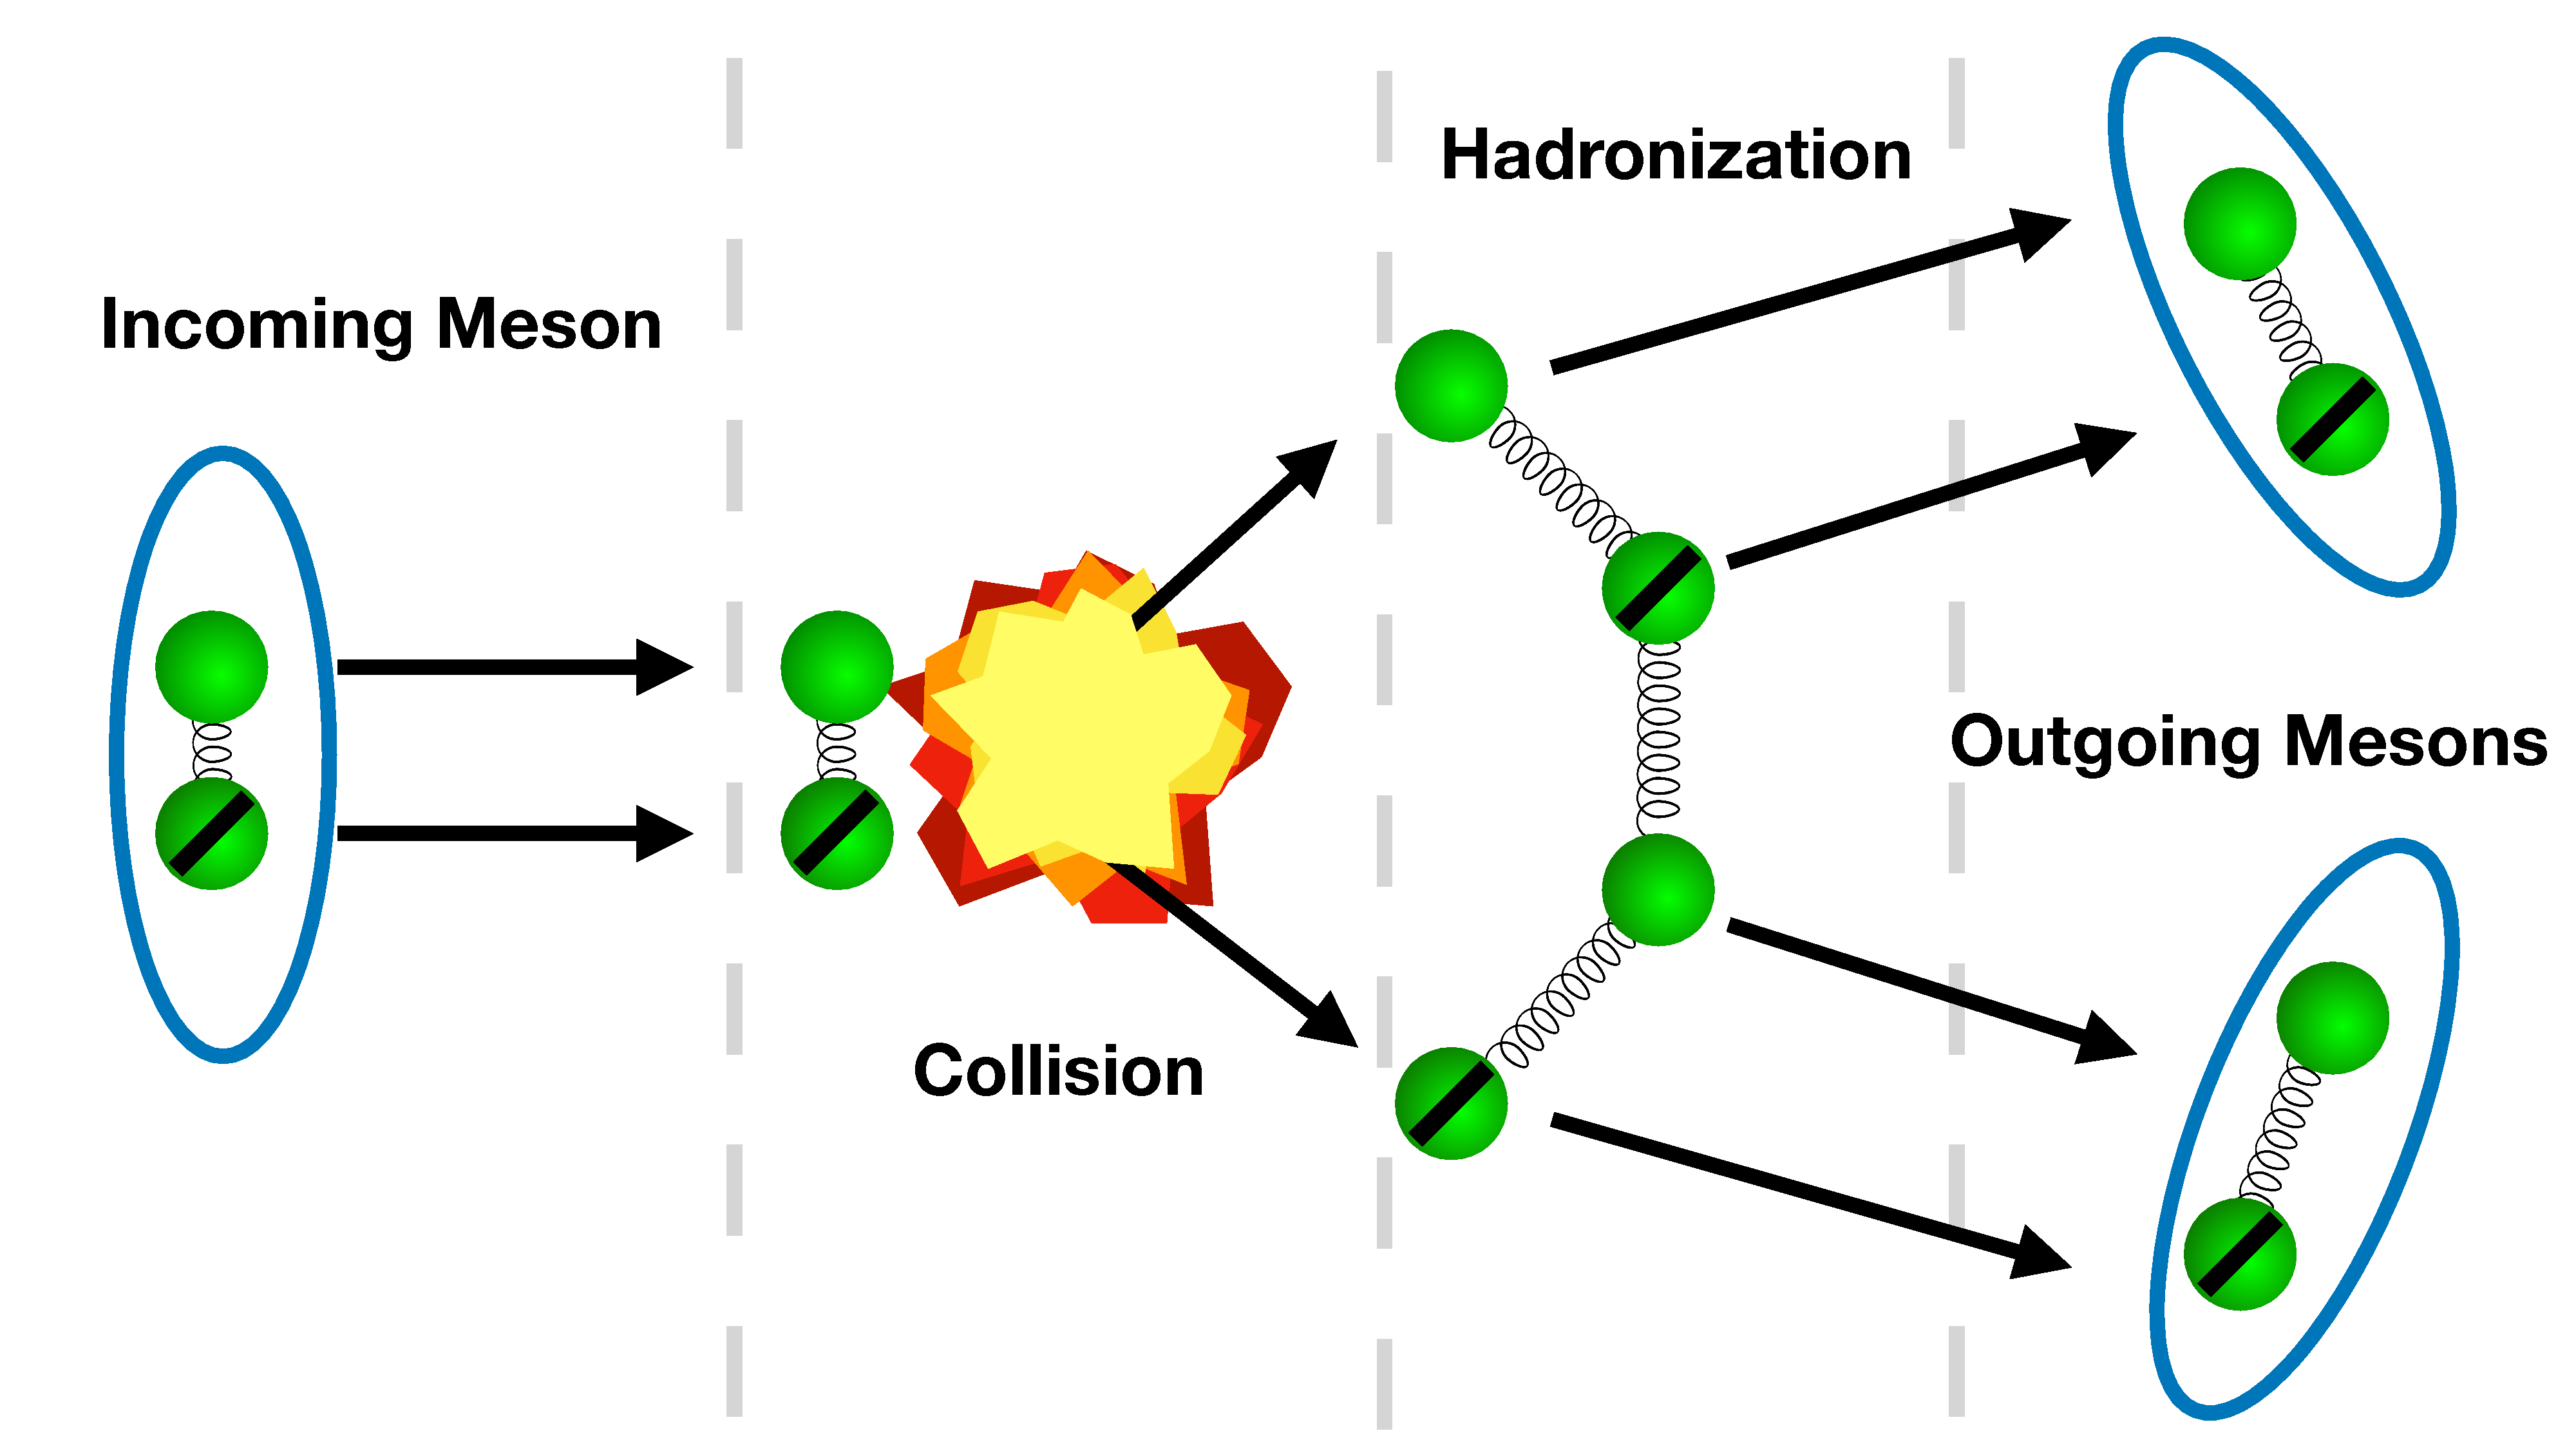
\includegraphics[width=\textwidth]{figures/hadronization.pdf}
    \caption[Hadronization of a meson.]
       {A simplified diagram of hadronization. In the collision, the quark and anti-quark of the meson acquire large kinetic energies relative to each other. As the meson's quarks begin to separate, the strong field strength between them increases. At some point, some of this energy is converted to make more quarks, splitting the meson in two.  This process continues until the kinetic energy of the originally \qqbar pair has been transferred to the rest mass and kinetic energy of multiple hadrons.}
    \label{fig:hadronization}
\end{figure}

\subsection{The Electroweak Interaction}
The electroweak interaction comes from the combination of two groups \SUtwoUone . This gives four vector bosons.  Three are from the \SUtwoL group: \ensuremath{A^i} with \ensuremath{i\in\{1,2,3\}}.  The last is from the \Uone group: \ensuremath{B}. The physical states observed, the W, Z and \ensuremath{\gamma} are linear combinations of \ensuremath{A^i} and \ensuremath{B}. These combinations define the W boson as
\begin{equation}\label{eq:Wboson}
    W_{\mu}^{\pm}
    \equiv  
    \frac{1}{\sqrt{2}}
    \left(
    A_{\mu}^{1}
    \pm
    iA_{\mu}^{2}
    \right)
\end{equation}
The Z and photon combinations are:
\begin{equation}\label{eq:Z}
    Z_{\mu}
    \equiv  
    \sin{\theta_W}
    B_{\mu}
    -
    \cos{\theta_W}
    A_\mu^3
    \end{equation}
\begin{equation}\label{eq:photon}
     A_{\mu}
    \equiv  
    \cos{\theta_W}
    B_{\mu}
    -
    \sin{\theta_W}
    A_\mu^3
\end{equation}

The \vminusa composition of the standard model weak force is parity-violating, and removes the possibility of right-handed weak interactions.  Thus, all neutrinos and all interactions with the W boson are only with left-handed particles. From the moment this theory was developed, physicists have worked at ways to restore parity symmetry with a right-handed weak interaction \cite{lr}\cite{lr1}.

\subsection{The Brout-Englert-Higgs Mechanism}
The Higgs mechanism takes a central role in the standard model. The Higgs field couples to every particle with mass in the standard model.  These interactions not only explain the mass of the electroweak bosons, which the Higgs mechanism is essential for, it also couples to fermions. The fermion mass term, in Weyl basis looks like this:
\begin{equation}\label{eq:higgs_fermion_mass}
\mathcal{L}_{D} = -m\bar{f}f = -m \chi _{L}^{\dagger}\chi _{R} - -m \chi _{R}^{\dagger}\chi _{L}.
\end{equation}
where $\chi _{L}$ and $\chi _{R}$ are left and right-handed component spinors of the fermion, $f$. This mass term is called the Dirac mass and used for all the massive fermions in the standard model. Neutrinos do not have a mass term in the standard model, and as they are exclusively left-handed, a mass term cannot simply be ``pencilled in''. The evidence for neutrino mass is extensive \cite{solar_neutrinos_davis}\cite{SNO_neutrinos} and requires new mass terms in the standard model. Left and right-handed neutrino masses are discussed further in section \ref{sec:seesaw}.

\section{Left-Right Symmetric Extensions to the Standard Model}
\label{sec:LRStheory}
The left-handed nature of the weak force \SUtwoL, and the left-right symmetry of every other group, leads to a desire to complete the symmetry of the standard model by adding a right-handed component to the weak force.  Completing the standard model has additional functional benefit in allowing for neutrinos to have a very light mass in a natural manner.  By the see-saw method, the currently observed left-handed neutrinos can be very light, countered by very heavy right-handed neutrinos. The symmetry would have to be broken at some energy level, allowing for the currently observed asymmetry at low energies.

Left-right symmetric extensions (LRS) models would require adding an additional symmetry group to the standard model or simply making the standard model a part of a larger symmetry like \SUfive or \Oten.  To simplify discussing the theory, we'll focus on the simplest extension.  Here, the electroweak sector simply gains another \SUtwo group, make it \SUlrs. Adding this extension creates three additional particles, the \WR and \NR, which are discussed in later in this chapter, and a partner to the \ensuremath{Z}, the \Zprime.  We will assume that left and right-handed interactions have the same coupling strength.  While this is not required in a more complicated LRS model, it provides a benchmark for the search. The right-handed extension additionally complicates the Higgs sector, requiring at least a Higgs doublet to couple to the right and left-handed weak bosons independently.

\subsection{See-saw Mechanism}
\label{sec:seesaw}
Left-right symmetric models provide a straightforward and natural mechanism for giving right and left-handed neutrinos mass. This mechanism is called the see-saw where one neutrino is very heavy and the other very light~\cite{neutrino_mass}. The see-saw Lagrangian combines Dirac and Majorana mass terms; Majorana mass terms only being possible for fermions without electric charge \cite{Majorana:1937vz}. 
\begin{equation}\label{eq:seesaw}
  \mathcal{L} = \frac{1}{2}
  \begin{pmatrix}
    \bar{\nu}_{Li} & \bar{\nu}_{Ri}
  \end{pmatrix}
  \begin{pmatrix}
    B'_{i} & M_{i} \\
    M_{i} & B_{i} 
  \end{pmatrix}
  \begin{pmatrix}
    \nu_{Li} \\
    \nu_{Ri}
  \end{pmatrix}.
\end{equation}
Each generation of neutrino is denoted by $i$. The terms $\nu_{R}$ and $\nu_{L}$ are pure left and right-handed spinors.  The $M$ is a Dirac mass component and gets its value from the vacuum expectation value of a LRS-Higgs field.  The $B'$ and $B$ masses are Majorana components and receive their mass from the individual left and right-handed LRS-Higgs doublets. With negligible mixing between generations, the mass eigenvalues are:
\begin{equation}
    \lambda_{+} \simeq B ,\ 
    \lambda_{-} \simeq -\frac{M^{2}}{B}.
\end{equation}
With $B \gg M$, which comes from that observation that $M_{W_{R}} \gg M_{W_{L}}$---if it exists. Now we can write the mass terms for the two observable neutrinos.
First with the mass eigenvalue of $\lambda_{-}$ we have the currently observed neutrinos.
\begin{equation}
\label{eq:light_neutrino}
    \nu \simeq
    \frac{1}{\sqrt{M^{2}+B^{2}}}\left(B\nu_{L} - M\nu_{R}\right)\simeq
    \nu_{L}-\frac{M}{B}\nu_{R}.
\end{equation}
It can be seen in equation \ref{eq:light_neutrino} that the right-handed spinor is a small component consistent with current observations. The heavy primarily right-handed neutrino state is then given as:
\begin{equation}
    N \simeq
    \frac{1}{\sqrt{M^{2}+B^{2}}}\left(M\nu_{L} + B\nu_{R}\right)\simeq
    \nu_{R}+\frac{M}{B}\nu_{L}.
\end{equation}

\subsection{Experimental Study of LRS Models}

While right-handed extensions to the weak force have been studied and sought for a long time, no specific experimental evidence exists for them.  In addition, the models themselves have too many free parameters to make any exact prediction.  Several different strategies can be emplyed.  Direct searches, where a new particle is produced on-shell and its decay products are seen, can probe for any of the additional particles predicted in LRS models.  Indirect searches, which look for subtle changes in known processes from additional or higher-order interactions involving a right-handed weak force, can also be done. The direct search for the \WR and \NR is the focus of this analysis. 
For a more detailed discussion of phenomenological constraints on the masses of right-handed weak force particles and their mixing see \cite{WRphenomLimits}.


\subsubsection{Direct Searches}
Any LRS model will include a new neutral-current boson, the \Zprime.  Perhaps the clearest signature of the existence of LRS interactions at the \LHC would be the \Zprime production and decay to leptons, \ZPtoLL. The heaviest standard model di-lepton resonance corresponds to the Z. As possible \Zprime masses are much higher than the Z mass, this region mass region would be relatively background free.  However, in a LRS model largely following the standard-model left-handed interaction, the \Zprime will be heavier than the \WR.  The \Zprime could be too heavy to produce at the \LHC, while the \WR could be quite visible.  Lower limits on the mass of the \Zprime have been set with this channel and are currently up to \SI{4.5}{\TeV} \cite{Zprime13TeVCMS}.

Direct searches for the \WR can be performed in a few different ways. One option would be focusing on the \WRtoLN\ decay. This search signature could be quite similar to a standard model W, assuming that the right-handed neutrino is relatively light and stable. However, right-handed neutrinos light enough to decay from a Z resonance would have played a role in the measurement of the well-constrained Z decay width. So, searches for this decay mode assume a heavy and decaying \NR, as this analysis does. 

The hadronic decay of the \WR, which would mirror the production mechanism we rely on, \WRtoQQ, can also be searched for.  It has a high branching fraction of the \WR decay and has no sensitivity to \NR mass, which can, as will be seen in this analysis, change the \WR decay topology significantly. However, the \WRtoQQ \xspace channel has significant QCD backgrounds, even in the highest masses reached at the \LHC, presenting a challenge for the search. Selecting the quark flavor in the decay and searching for \WRtoTB\xspace can be done, and would reduce the amount of QCD. The top produced in the \WR decay can decay producing leptons which would give a better handle on the study than a generic jet search, though with a cost in branching ratio. Searches for heavy di-jet resonances have been performed at \CMS with the most recent search using the same years as this analysis.  These searches can exclude many different signal models, including the \WR.  Masses of a di-jet resonance similar to the \WR were excluded up to \SI{3.6}{\TeV} \cite{dijetRunIICMS}.  A third \WR signature to search for relies on a possible beyond-the-standard-model behavior where some LRS models create a doubly charged \WR. This decay, which produces two leptons of the same sign, is very unique from the standard model and can be also be searched for. The most recent search was performed by the ATLAS collaboration, setting a limit at \ensuremath{\SI{4.7}{\TeV}} \cite{ATLASresWR}.

\subsubsection{Indirect Searches}
Direct searches provide an obvious way of finding new particles. However, any LRS extensions would also affect standard model processes and constants through additional virtual interactions with the new particles. There are many examples of this: exotic behaviors like neutrino-less double beta decay, left-right mixing, or even lepton-flavor violation could occur. The lack of observation for these behaviors up to date would need to be explained by their having an exceptionally low rate, which can be acheived by the new particles having masses $\gtrapprox \SI{2}{\TeV}$. An LRS model could also affect currently understood behaviors, but to a degree too small to be yet measured.  The electron electric dipole and neutron meson mixing and mass difference are examples of this.  Measurements of all of these, or upper limits on possible rates of processes not in the standard model, provide additional limits which can constrain the search area for direct searches.  The best interaction to study for an indirect search, or limit, on LRS models is with neutral mesons.  The mixing of neutral meson states---and their mass---are affected by CP-violation.

\begin{figure}[!btp]
    \centering
    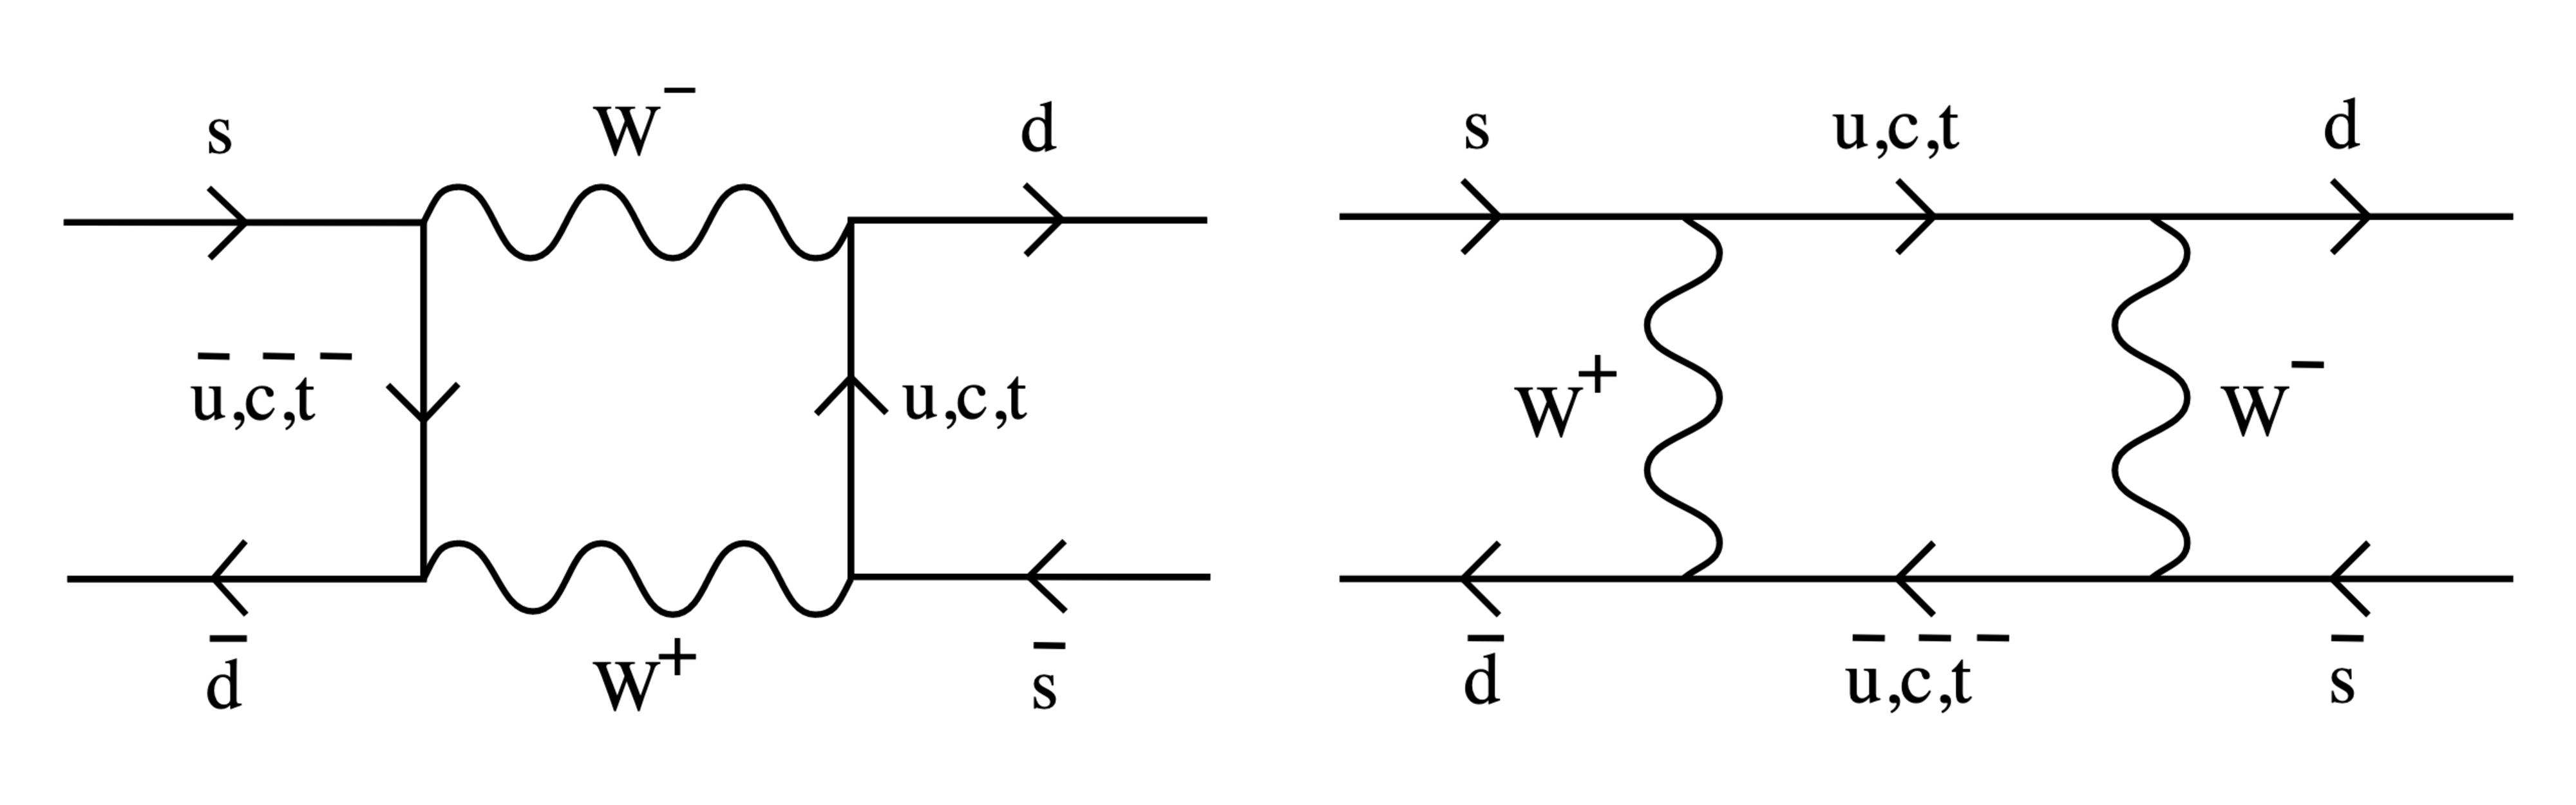
\includegraphics[width=\textwidth]{figures/kaons.pdf}
    \caption[Kaon mixing diagrams]
       {The two leading kaon mixing diagrams are shown here. As quarks occur naturally left and right-handed, a virtual \WR would be contribute identical diagrams to this process \cite{kaon_mixing}.}
    \label{fig:kaon_mixing}
\end{figure}

Neutral Kaons are mesons, composites of two quarks, made of one strange and one down quark.  One or the other will be an anti-particle, with the particle being the down and anti-strange combination.  Physically-propagating neutral Kaon states are neither, but two different combinations of the Kaon and anti-Kaon.  These are called K short and K long, based on the striking observation that one (the K long) has a much longer lifetime than the K short, and can be observed to travel in the lab frame.  This mixing of \ensuremath{K_0} and \ensuremath{\Bar{K_0}} comes from CP-violation.  This mixing involves a diagram with the exchange of two W bosons. If there is a \WR, this diagram exists not just for the standard model W but also the right-handed W boson, as quarks can be right and left-handed.  This increases the mixing, but is also heavily dependent on the mass of the \WR.  The heavier the \WR, the less significant its contribution. Precision measurements of Kaon mixing allow for a lower limit on the \WR mass to be set at \SI{2.5}{\TeV} \cite{left_right_LHC}.

\section{New Particle Production at the LHC and PDF Effects}
As the highest energy particle collider created to date, the LHC has the possibility to reach collision energy levels where new, previously unobserved particles could be created.  Descriptions of the \LHC and \CMS are in Chapter \ref{experiment_chapter}.  As this analysis is a direct search for particles beyond the standard model, its important to review the way in which the \LHC generates high mass particles. An overview of the rates of different standard model interactions, and hypothesized beyond the stand model interactions are shown in Fig:~\ref{fig:lhc_rates}. The cross-sections searched in this analysis vary, but in the upper-most mass limit are on the order of a femtobarn, which as can be seen in the figure, occur no more than several times a year.

\begin{figure}[!btp]
    \centering
    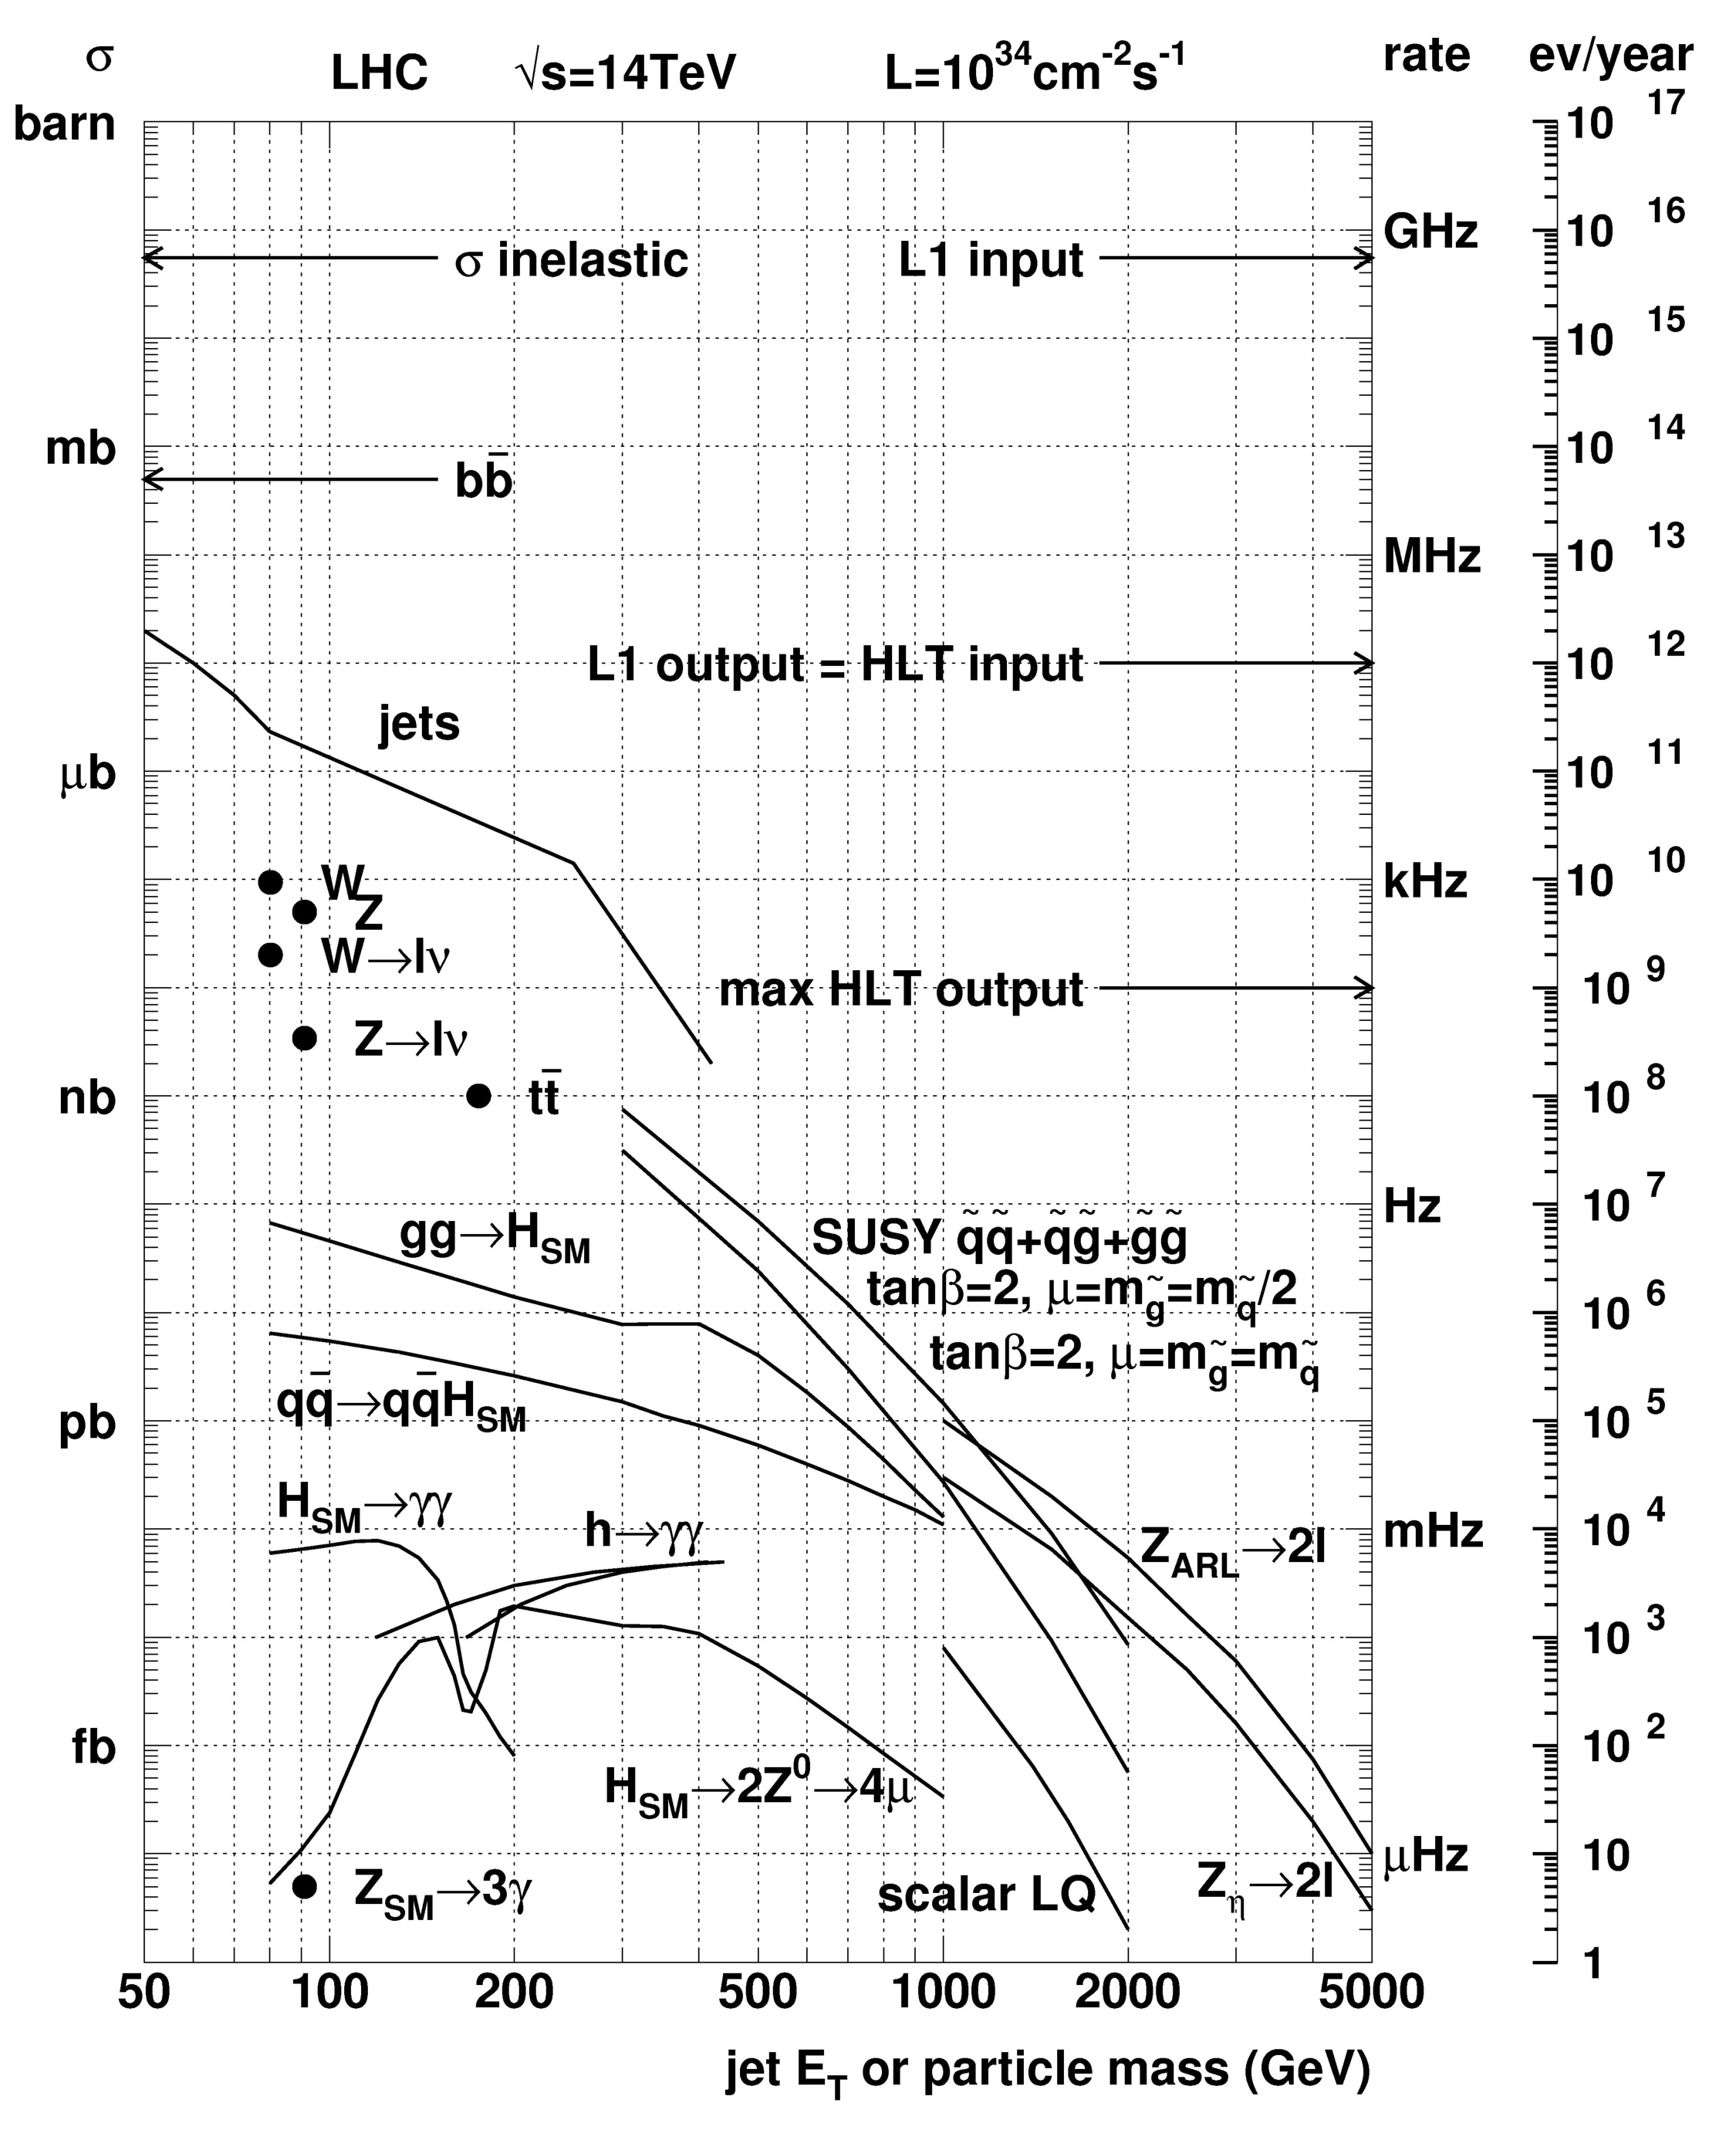
\includegraphics[width=\textwidth]{figures/lhc_rates.pdf}
    \caption[Interaction rates at the \LHC.]
       {Interaction rates for various standard model and theorized beyond the standard model processes are shown.  From top to bottom interactions occur at lower and lower rates until, below the inverse-femtobarn level, they would not be expected to occur at the \LHC \cite{lhc_rates}.}
    \label{fig:lhc_rates}
\end{figure}


\subsection{Parton Density Functions and Proton-proton Collisions}
Collisions at the \LHC take place between protons. Each proton carries with it three quarks and a large amount of QCD potential energy, which manifests as a combination of gluons and short-lived quark and anti-quak pairs of all flavors. Actual interactions occur between these parts of the proton, called ``partons''. In theory, any quark or gluon can interact in the proton-proton collision. The amount of momentum carried by an interacting parton varies according the amount of momentum exchanged in the collision, always less than the total collision energy of \rootsthirteen. Thus, any particle produced at the \LHC must have a mass substantially smaller than \ensuremath{\SI{13}{\TeV}}. Figure~\ref{fig:proton_pdfs} shows the relationship between parton interaction probabilities and momentum exchanged in collision for varying collision energies. The extremely heavy \WR would mostly be produced in a collision between a valence quark, and a sea anti-quark. However, many of the most frequent standard model boson production modes involve gluons at \LHC energies.
\begin{figure}[!btp]
    \centering
    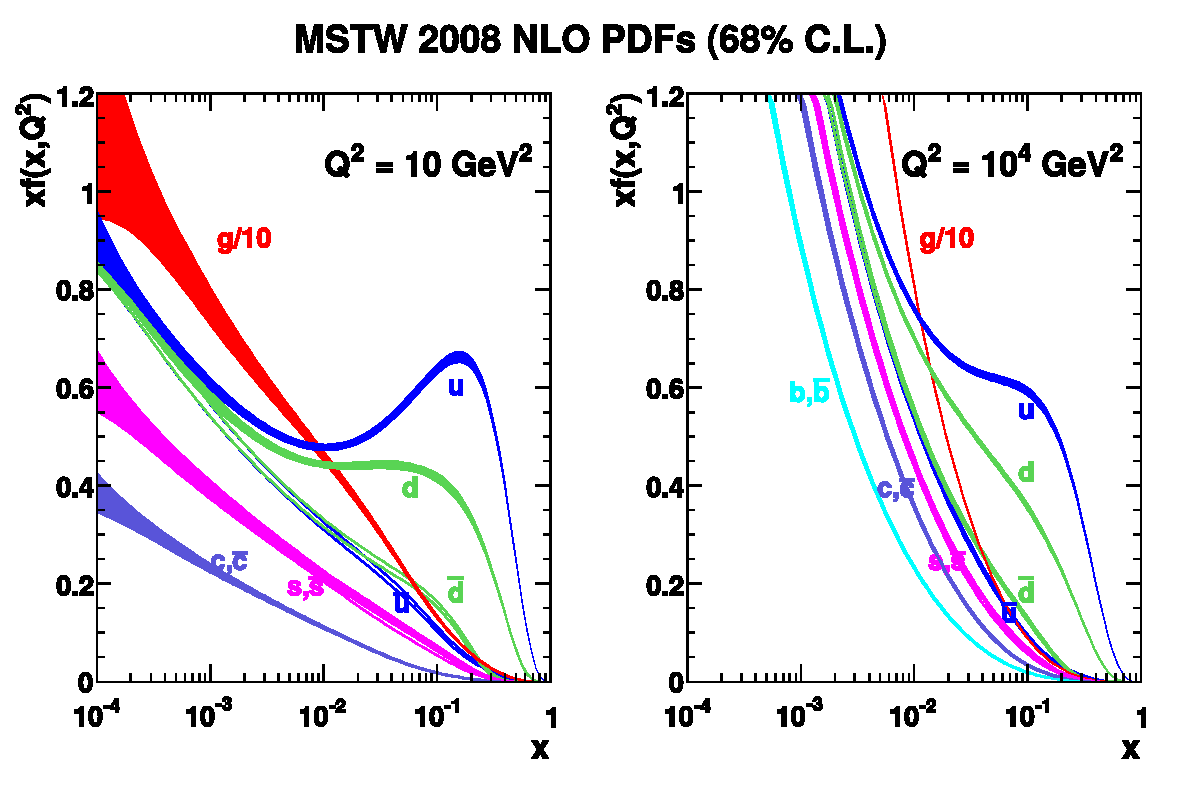
\includegraphics[width=\textwidth]{figures/mstw_pdfs.pdf}
    \caption[Proton PDFs at the \LHC]
       {Two sets of parton density functions (PDFs) are presented here. A collision at lower energies is shown on the left, and a higher energy collision, more relevant to \WR production is shown on the right. While the variables $xf$, $x$, and $Q^2$ are beyond the scope of this chapter, the y-axis can be interpreted as the rough probability of interaction, and the x-axis the momentum fraction exchanged in collision. At high momentum fractions (toward the left and as required by a heavy \WR) the shell quarks of a protons are seen to dominate. At lower momentum fractions (as would occur with standard model particle production at the \LHC) gluons dominate \cite{PDFExample}}. 
       %The top and bottom quark PDFs are conspicuously absent as they do not have a well measured PDF.
    \label{fig:proton_pdfs}
\end{figure}

In every high energy particle collision, the energy of the collision available to produce new particle mass is defined as:
\begin{equation}\label{eq:roots}
    \sqrt[]{s}
    =   
    \sqrt[]{
       \left( \sum_{i=1}^{2} E_i \right) ^ 2
       -
       \left( \sum_{i=1}^{2} \boldmath{p}_i \right) ^ 2
    }
\end{equation}

All particle creation at the \LHC must obey the relation in Eq.~\ref{eq:roots}, however, particles lighter than this relationship receive an additional bonus from having additional momentum phase-space to be produced in. Extremely heavy particles, like the \WR will generally be produced close to at rest in the lab frame as a result.

As a result of the parton momentum exchange probabilities, this analysis only searches for particles up to a mass of \ensuremath{\SI{7}{\TeV}}, and is only successful  in setting a limit at less than \ensuremath{\SI{6}{\TeV}}.  Heavier particles (even particles with a mass higher than \ensuremath{\SI{13}{\TeV}}) can be searched for at the \LHC, but they will be increasingly virtual in interaction at the \LHC as their resonant mass increases. These are very challenging to search for, as they present as a broad excess, rather than a peaking, resonant, mass distribution.

\subsubsection{\WRNR mass effects at the \LHC}
While this analysis can be colloquially referred to as a ``bump hunt'', the shape of the \WR mass spectrum in our selection can stretch beyond a typical resonant peak. This analysis exclusively seeks \WR events which decay to on-shell right-handed neutrinos. This necessarily truncates the \WR mass spectrum to be produced above the \NR mass generated. In the lower \NR mass boosted regime, the \WR mass spectrum is less and less truncated, opening up the possibility of low-mass offshell \WR events to be produced. These events are enhanced by the steeply falling probability of collisions at higher mass. The full shape of the generated \WR mass is shown in Fig.~\ref{fig:wr_5000_100_spectrum} at one of the \WRNR mass points where the off-shell contribution is most notable.
\label{sec:WRshape}
 \begin{figure}[!btp]
    \centering
    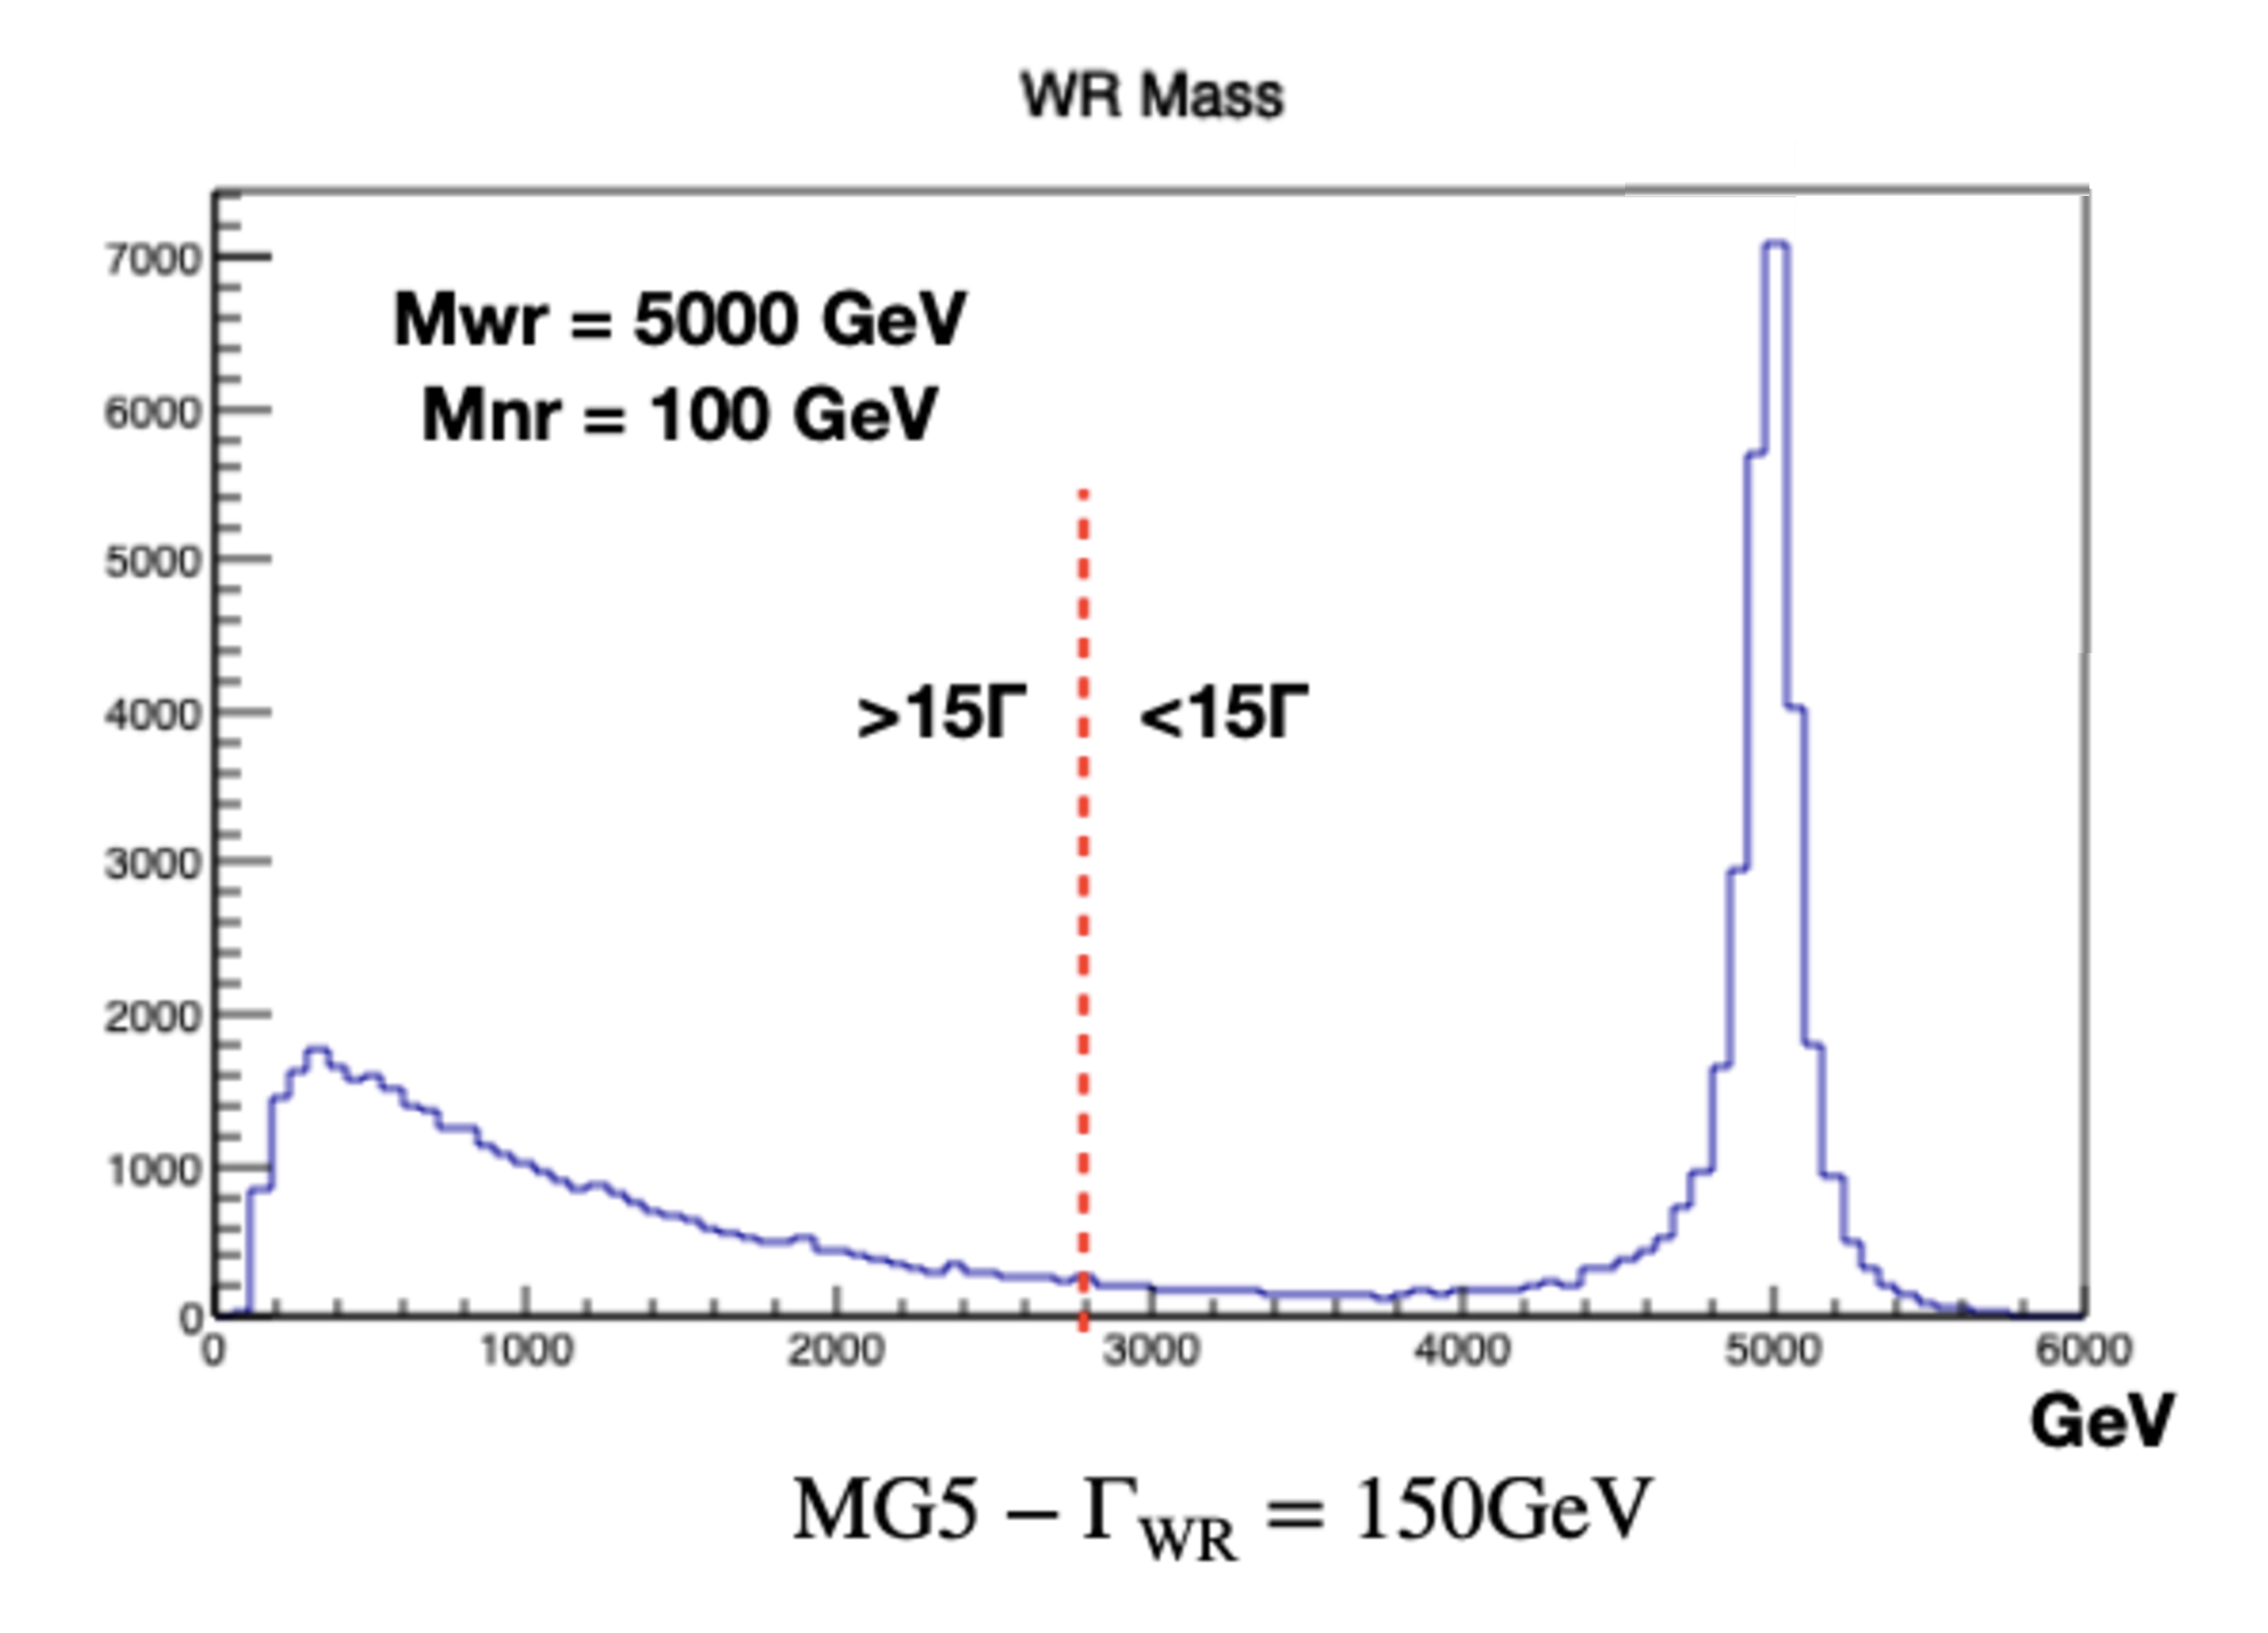
\includegraphics[width=\textwidth]{figures/WR_5000_100_spectrum.pdf}
    \caption[\WR mass spectrum]
       {The generated mass spectrum for a \WRNR mass of 5000-100. The on-shell/off-shell cutoff configured in the Monte-Carlo generator is shown as well and corresponds to 15 times the natural width of the \WR. It can be seen that nearly half of the generated \WR events fall below the cutoff.
       }. 
       %The top and bottom quark PDFs are conspicuously absent as they do not have a well measured PDF.
    \label{fig:wr_5000_100_spectrum}
\end{figure}
%%%%%%%%%%%%%%%%%%%%%%%%%%%%%%%%%%%%%%%%%%%%%%%%%%%%%%%%%%%%%%%%%%%%%%%%%%%%%%%%

%%%%%%%%%%%%%%%%%%%%%%%%%%%%%%%%%%%%%%%%%%%%%%%%%%%%%%%%%%%%%%%%%%%%%%%%%%%%%%%%
